% !TeX root = ../INTO-CPS-Manifesto.tex

\section{The INTO-CPS Industrial Case Studies}\label{sec:casestudies}

%\fbox{Stylianos Basagiannis}

The industrial domains benefited from the INTO-CPS technologies in different ways, as expected due to their different multidisciplinary engineering activities. Nonetheless, certain aspects of the tool chain were of benefit to all industrial partners. We thus argue that these are the most broadly applicable benefits of INTO-CPS and the ones that can most successfully be transferred to other domains (fig.~\ref{fig:industrial}).
Modelling and simulation is heavily used in industry today, to evaluate performance and robustness of the system with regards to requirements. Aspects such as simulation speed, and model fidelity are of high importance. Going beyond model-based design and single model simulation, co-simulation enables the analysis of physical interactions of systems that were previously not captured, due to the different domains at which the physics were modelled. Multi-physics analysis enables early analysis and detection of issues that were only uncovered at the physical prototyping stage, thus saving time and money.

The use of SysML modelling with the INTO-CPS profile was valuable to the majority of the industrial case studies, as a way to provide a common documentation of the system structure (particularly valuable for larger teams). It also enhanced communication within each case study project and across the disciplines and tools of the project. The connection with the simulation tools and the COE via the export of Model Description and Co-Simulation Configuration adds even more value to the SysML model.
The DSE component was valuable as a way to sweep parameters and automate co-simulations. This led to faster prototyping (and lessened the need for physical prototypes) and a better understanding of the complex interactions between the system parameters. The DSE component was well integrated into the toolchain and used in the industrial studies through a user friendly interface, providing also its capability to reuse existing parts of the tools and models (through respectively the INTO-CPS application and FMUs).

\begin{figure}[!ht]
	\centering
		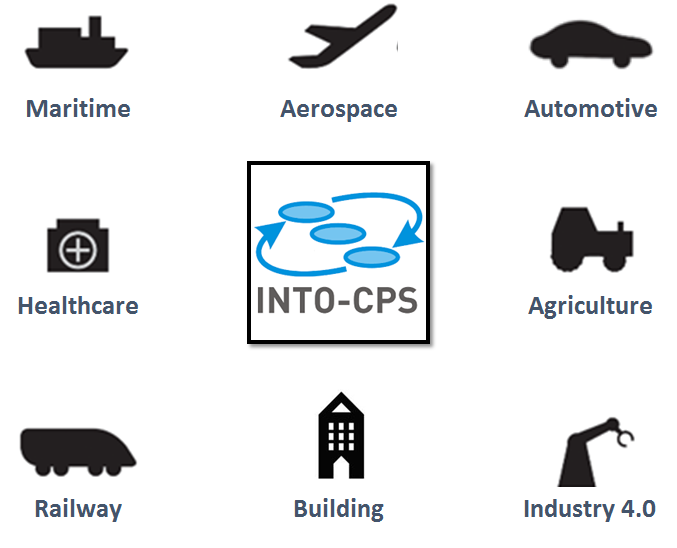
\includegraphics[width=0.5 \textwidth]{./figures/industrial}
	\caption{INTO-CPS Industrial Case studies}
	\label{fig:industrial}
\end{figure}

The 3D visualisation component was valuable for all industrial partners. As commercial entities, the 3D visualisation has great value as a marketing and sales tool. It also greatly enhances the user experience when analysing the models. These benefits are in addition to engineering benefits which can be gained for certain case studies, where the visual aspects of the problem are of interest and can be studied using the 3D visualisation. This is not the case for all CPS problems, but any CPS company can benefit from the 3D capabilities for marketing purposes, which are of high importance to any business. More generally, one of the greater benefits of the INTO-CPS tool chain was the ability to reuse models, including existing legacy models for new purposes. The broad tool compatibility (including tools outside the tool chain, this attesting its openness) increased the reuse even more. The tool chain is also fully compliant with the FMI standard which increases the value of models developed with the INTO-CPS tool chain, as they can be reused further in the future. Finally, the baseline tools of INTO-CPS were all made compatible and tested with industry-grade and open source tools through the FMI standard, thus opening new possibilities for the tools and their users.

\subsection{The Automotive Case Study} 

This sections presents mainly a case study that develops functions for vehicles, in particular electric vehicles using the INTO-CPS technology. Its goal is to create an assistant system for estimating the range of an electric vehicle, based on a vehicle model and real data from the environment, such as route topology or weather. Furthermore, the range estimation is dynamic, as it takes changes in the initial assumptions into account, and influences the vehicle behaviour accordingly. 

\begin{figure}[!ht]
	\centering
		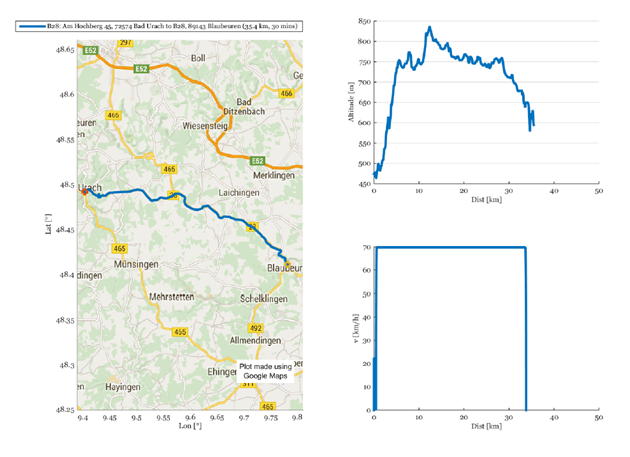
\includegraphics[width=0.9 \textwidth]{./figures/auto}
	\caption{Automotive case study using INTO-CPS: Velocity and altitude profile for a route of 35 km in the vicinity of Stuttgart. The route consists here of a country road only, and thus the velocity is stable at 70 km/h, while the altitude varies between 450m and 850m above sea level.}
	\label{fig:auto}
\end{figure}

The case study can be considered a CPS because it contains local intelligence and autonomy in the vehicle. This is assisted by information about its environment typically derived from a cloud context (here, information on weather and traffic / route) and the logic depends upon the physical dynamics of the electric vehicle (Fig.~\ref{fig:auto}). 

A part of the system is transferred seamlessly from a simulation model to real hardware (here, as Raspberry Pi) and simulated with the remainder of the system. Since the case study was developed as part of the INTO-CPS project \cite{Fitzgerald&15,Larsen&16a,Larsen&16c,Larsen&16e,Larsen&17a}, one aim was to evaluate the INTO-CPS tools and methods. Here this is in particular the Co-simulation orchestration engine (COE), which is a FMI 2.0 compliant master algorithm that allows coupling of continuous-time (CT) and discrete event (DE) models in a Co-Simulation setup [4,5].  furthermore, the system was modelled in SysML, using the CPS-extension of the Modelio tools \cite{Bagnato&15}. The models themselves were created using Matlab\footnote{\url{https://www.mathworks.com/products/matlab.html}}, 20-sim\footnote{\url{http://www.20sim.com/}} \cite{Kleijn06}, C++ and Overture\footnote{\url{http://overturetool.org/}} \cite{Larsen&10a}.

\subsection{The Agricultural Case Study} 

The focus of the case study is the development of the agricultural field robot, Robotti using the INTO-CPS technology. Models of the machine dynamics and controllers have been developed using the baseline tools and Co-simulated using the COE. The DSE feature is applied in the development and assessment of the steering controller which is crucial to the performance of the robot. The agricultural case study has been extended with an additional industrial application, namely the AI-Mower. The dynamics of the mower is modelled and co-simulated to assess and optimise a new approach for steering the mower. 

\begin{figure}[!ht]
	\centering
		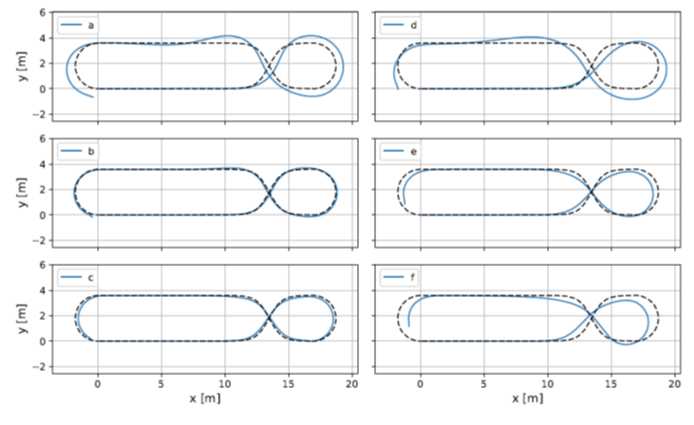
\includegraphics[width=0.9 \textwidth]{./figures/agri}
	\caption{Simulated trajectories of the six controller configurations (a,b,...,f)}
	\label{fig:agri}
\end{figure}

Additionally, the 3D FMU feature has been applied to visualise the machine based on the models of the kinematics and dynamics. The details on the mower are kept confidential contrary to the Robotti project which is public.
Through the model development using INTO-CPS, the work related to Robotti have been focused towards DSE-based optimisation of the steering controller which is crucial to the performance of the machine. Several scenarios of different steering controller configurations are simulated using the COE and the DSE feature is applied to estimate the optimal controller configuration of the Robotti. The influence of the controller parameters are shown in Fig.~\ref{fig:agri} where the six simulated trajectories are shown corresponding to six combinations of two controller parameters. The dashed line represents the desired route and the blue line represents the simulated trajectory of the Robot.

Related Publications can be found at \cite{Foldager&17}.


\subsection{The Building Case Study } 
 The building case study focuses on modelling and analysis of energy and comfort for Heating, Ventilation and Air Conditioning (HVAC) systems that control the temperature of connected areas inside building premises. The case study models various concepts shown in fig. \ref{fig:building} such as: a) Fan Coil Unit (FCU) and control; b) Supervision and fault detection of FCUs; c) Communication between master-slave FCUs; d) Communication between FCUs and supervisor; e) Air Handling Unit (AHU) and control; f) Chiller load and control; g) Physical rooms and air flow; h) Water and air pipe connections.

The functionality of the HVAC is to regulate operation of various devices to ensure user comfort. User inputs are taken into account from room and zone thermostats and are compared with current Room Air Temperature (RAT) sensed by the FCUs, triggering certain action on the FCUs to reach the desired temperature by a) regulating the air flow using its fan, b) regulating the water pipe valves to control the cooled water into the coil, c) synchronising with the supervisor to coordinate with the rest of the FCUs. Fresh air is provided to the FCUs by the AHU and cooled by the Chiller.

\begin{figure}[!ht]
	\centering
		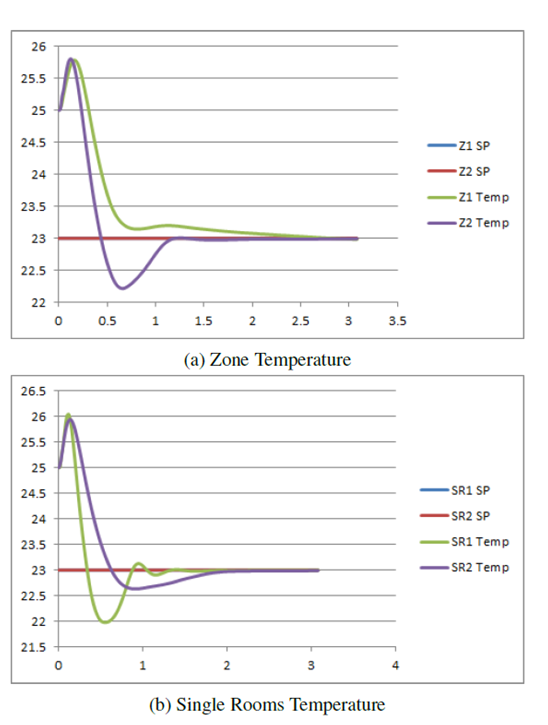
\includegraphics[width=0.9 \textwidth]{./figures/building}
	\caption{INTO-CPS Co-Simulation Results for Room temperature in building zones}
	\label{fig:building}
\end{figure}

Modelling and simulation is heavily used to evaluate performance and robustness of the system with regards to requirements. Aspects such as simulation speed, and model fidelity are of high importance. Going beyond model-based design and single model simulation, co-simulation enables the analysis of physical interactions of systems that were previously not captured, due to the different domains at which the physics were modelled. Multi-physics analysis enables early analysis and detection of issues that were only uncovered at the physical prototyping stage, thus saving time and money. The 3D visualisation feature is particularly appealing for several spatial exploration of HVACs effectiveness, as well as for engaging with non-technical stakeholders and demonstrating results. In addition, certain industrial domains operate in context where the visual aspect of the 3D co-simulation can bring genuine insights. Other capabilities of the INTO-CPS tool chain such as test automation and verification are not particularly in demand for HVAC systems, but are highly valuable for aerospace applications.

Related Publications can be found at \cite{Fitzgerald&16,Couto&17}.

\subsection{The Railway case study} 

In railway signalling, an interlocking is an arrangement of signal apparatus that prevents conflicting movements of trains through an arrangement of tracks, junctions and crossings. Usually, interlocking is in charge of a complete railways or tram line, computing the status of actuators (switches and signals) based on signalling safety rules that are encoded as ``binary equations'' as shown in Figure 2, usually managing s 180.000 equations that have to be recalculated several times per second. These equations compute the commands to be issued to track-side devices: they encode the safety behaviour that enable trains to move from one position to another through routes that are allocated and then released. Currently, there are attempts to find the right trade-off between efficiency of an interlocking system (availability of routes, trains' delays and cost of interlocking system) and safety (collision avoidance, derailment prevention, availability and efficiency of emergency system).

In this case study, an Interlocking system was considered that controls a part of a tramway line, including two platforms and a bidirectional track (between SW5 and SW2). It involves eleven track circuits; sensors that detect the absence of a train on a railway track; three commands that can accept several positions and are activated by the train; five mechanical switches that allow changing direction (those switches have to be set accordingly to the route chosen) and three light signals, red when the train is not allowed on the track and green when it can pass. The interlocking system also makes use of five mechanical safety relays that externalise the state of a route and allow redundancy between software logic and electronic circuits.

Related Publications can be found at~\cite{Larsen&16d}

\subsection{The Aerospace case study} 
IDA2- Aerospace - MISSION


\subsection{Integrated product-production co-simulation for cyber-physical production system (iPP4CPPS) } 

The case study involved the virtual design and validation of a CPS-based manufacturing system for assembling USB sticks, inspired from Continental's real manufacturing and testing processes in a production line. It is a representative example of distributed heterogeneous systems in which products, manufacturing resources, orders and infrastructure are all cyber-physical. In this setting, several features (such as asynchronous communication, messages flow, autonomy, self-adaptation, etc.) could be investigated at design time, for example using a collaborative modelling approach. Consequently, the case study offered a balance between being sufficiently simple to be easily followed as a production line example, including generating a tangible output, and at the same time being sufficiently general to allow the study of the co-simulation complexity. Furthermore, by choosing a USB stick, the example opened the (unexplored) possibility of extending the purpose of the study to interactions between generated hardware and generated software solutions in the production line.

Obviously, this small experiment, in terms of scale and time, could not give a full and clear assessment of benefits for developing an integrated product-production co-simulation for CPS-based industrial control. Nevertheless, there were some recognisable benefits compared to the current state of technology:

\begin{itemize}
\item the possibility to simulate, test and validate from a holistic perspective and with an increased level of accuracy an entire production system that needs cross-functional expertise; The initial development of a homogeneous co-simulation in VDM for the iPP4CPPS prototype was particularly useful in driving cooperation and making clear the assumptions of the distributed teams involved in modelling the specific components. This phase proved to be the most difficult and time-consuming in building the co-simulation, requiring a very intensive communication for a shared understating of the requirements. Once the VDM co-simulation was running, the independent developments of units could be integrated, validated and deployed in any order.
\item to a certain extent, the ability to handle unpredictable integration requirements. The employment of co-simulations when designing an automated production system avoided the build-up inertia of subsequent design constraints, facilitating the low and late commitment for these decisions, i.e.\ the specific micro-controllers or PLCs, the layout of the plant, the number of memory boxes from the warehouse etc. For example, the possibility to generate code - from all the simulation tools used in this experiment (i.e.\ 4DIAC, 20-Sim, Overture) -- for an extended set of computational devices was a clear advantage in respect to late commitment for the computational system used in the production system. 
\end{itemize}

The methodology adopted in the IPP4CPPS project to develop the co-simulation closely followed the classical stages of agent-oriented or component-based software engineering methodologies. Following the mechanical model derived from the requirements, the high-level abstraction for the behaviour of each simulation was implemented and the interactions among the components could be analysed. It included distinct simulations for each component type (Table 1): production (i.e.\ warehouse station, robot, transporting wagons, and testing station), orders (i.e.\ placed via mobile devices), and factory infrastructure (i.e.\ part tracker). 

The co-simulation model had been initially implemented in VDM and validated on the INTO-CPS tools chain. The main goal of this implementation was manifold: a) to validate the interaction protocols among the composite simulations; b) to have an early working co-simulation where the specific simulations may be gradually added, tested and validated; c) to allow for a more independent development among the dispersed teams involved in modelling the specific simulations, while at the same time keeping the co-simulation functional at all times; and d) to cover the left-over parts of the co-simulation whose modelling was not needed in detail for the validation of the interaction protocol (e.g.\ test station) or for which there is was FMI-compliant tool (i.e.\ factory infrastructure).   

\begin{table*}[ht]
	\centering
		\begin{tabular}{|p{2.4cm}|p{1.8cm}|p{3.2cm}|p{4cm}|}\hline
			\textbf{Component type} & \textbf{Unit} & \textbf{Technology} & \textbf{Deployment}\\
			\hline\hline
			Orders & HMI & 4DIAC + MQTT \textit{or} Overture (VDM) & smartphones and tablets \\ \hline
			Infrastructure & Part Tracker & Overture (VDM) & NVIDIA Tegra Jetson\\ \hline
			Production & Warehouse + Robotic Arm & 20-sim & Raspberry Pi with UniPi Expansion Board + Stäubli robot\\ \hline
			Production & Wagons & 4DIAC & Raspberry Pi controlling DC motors, position sensors and anti-collision ultrasonic sensors \\ \hline
			Production & Test Station & 4DIAC & Cognex Vision Insight 1100 camera connected to Raspberry Pi for actuators control\\ \hline
			General & Unity & 20-sim animation & PC\\\hline
		\end{tabular}
	\caption{Technologies used for different system components}
	\label{tab:iPP4CPPS_technologies}
\end{table*}

The detailed model of each simulation covered a continuous-time model realised in 20-Sim for the warehouse and robotic arm, a discrete-time model in 4DIAC for the transportation system and test station, and a discrete-time model in Overture for the infrastructure. All units modelled and tested by the heterogeneous co-simulation were then deployed in a demo stand for fine tuning under real-life conditions (Table \ref{tab:iPP4CPPS_technologies}). This phase presumed the extension of code generation capabilities of the simulation tools, such as: 20-sim 4C has been extended with MQTT, Modbus, I2C colour sensor, I2C multiplexer and UniPi board for the Raspberry Pi; Overture for employing MQTT as communication protocol on a Raspberry Pi 3; and 4DIAC for accelerometers control. 

\begin{figure}[!ht]
	\centering
		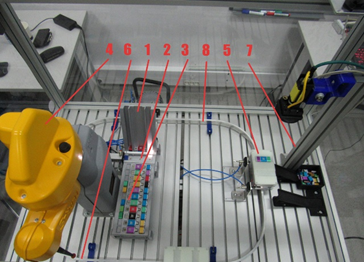
\includegraphics[width=0.9 \textwidth]{./figures/demo_stand}
	\caption{Demo stand for deployment of the co-simulated units, containing: 1) the warehouse stacks; 2) the assembly box at the base of the warehouse stacks; 3) the memory boxes of the warehouse unit; 4) the robotic arm for moving parts around the warehouse; 5) wagons on different locations of the track; 6) the loading station; 7) the test station; 8) the circular track for the wagons..}
	\label{fig:demo_stand}
\end{figure}

The experiment assessed the benefits and the maturity level of model-driven engineering technologies for future adoption into CPS-based production systems. It covered the entire engineering life-cycle (i.e. from requirements to deployment into a real infrastructure) and contributed to several advancements of engineering methods and tools. The experiment delivered an effective proof-of-concept for model-driven engineering of CPS-based production system as a feasible and promising approach to (re)engineer the factory of the future with the employed technologies (i.e.\ INTO-CPS, Overture, 20-Sim and 4DIAC). Nevertheless, the experiment also identified a number of issues that may have further impact over the adoption of model-driven engineering technologies into real settings: the FMI-compatibility of the simulation tools used in industry; the hardware/software-in-the-loop simulations still display complex synchronisation problems for dissimilar time-scales; the extended set of low-level devices (i.e.\ sensors, industrial communication standards etc.) that are used in today and future industry require special standardisation effort to enhance the deployment capabilities of the simulation tools\footnote{More information can be found at \url{http://centers.ulbsibiu.ro/incon/index.php/ipp4cpps/} and \url{http://www.cpse-labs.eu/experiment.php?id=c3_uk_gs_ipp4cpps}.}

\subsection{Use of the INTO-CPS Technology at MAN Diesel \& Turbo}

As reported in \cite{Pedersen&17}, at \ac{mdt} the conventional approach for
developing two-stroke combustion engines with a distributed embedded control
system is being challenged. In particular, for diesel engines pollution is a
key element that it is desirable to reduce from a competitive perspective. New
emission legislation focuses on the reduction of especially NO$_x$ emission.
Widely known emission reduction technologies for reducing NO$_x$ are selective
catalytic reduction and \ac{egr}, both being developed at \ac{mdt}
\cite{Pedersen&17}.

These systems require advanced algorithms to control the complexity of the
physical dynamics of large engines. \ac{mdt} is divided into different
departments with different responsibilities in the same way as many other large
organisations. In the control department at \ac{mdt}, control algorithms are
created directly in the target software framework with the possibility of
performing \ac{sil} simulation during development.  Models of the physical
behaviour are created in other departments of \ac{mdt} using the tools most
suitable for the specific constituent system.  

For the control system development, the physical dynamics models are
implemented in an internally developed tool for \ac{ct} simulation called the
\ac{mdse} which is part of the software framework. The primary focus in
\ac{mdse} is \ac{sil}/\ac{hil}, and the physics models implemented here are
often an abstraction of high-fidelity models. Historically it has been
challenging inside \ac{mdt} to enable heterogeneous collaborations between the
different teams producing models in different departments. As a result
different models are typically fragmented and solely used within one department
for the dedicated purpose each of the models serve. Thus, efforts that goes
across these individual insights are only found at the test on the real
platform.


%% Change this paragraph
At \ac{mdt} the models used in the control department are based on a software
framework and \ac{mdse} is implemented in C++ and run on a 32-bit Linux
platform while the physical modelling tools often require Windows. During the
INTO-CPS project it was illustrated how a transition from the current
simulation process at \ac{mdt} to one using co-simulation utilising the
\ac{fmi} standard can be performed by using the \ac{coe} from the \ac{intocps}
project. 

The aim with the approach suggested was to reduce redundancy in the
development process and reuse and combine models from different
departments \cite{Pedersen&17}. One of the main challenges for such a transition
is to enable co-simulation across different hardware architectures and \ac{os}
platforms due to constraints from software frameworks, physical simulation
tools and version compatibility, and INTO-CPS Technology was key in overcoming
it.

\subsection{Use of the INTO-CPS Technology at the European Space Agency}


At the European Space Agency (ESA) many systems fall into the CPS category.  As
reported in \cite{Feo-Arenis&17}, the Mars Rover case study, which was
developed in Crescendo, a previous project, had been restricted to the
combination of two models:  one Discrete Event (DE) model expressed using the
Vienna Development Method (VDM) \cite{Fitzgerald&08c} using the Overture tool
\cite{Larsen&10a} and one Continuous-Time (CT) model expressed using bond graphs
\cite{Karnopp&68} and the 20-sim tool \cite{Kleijn06}. 

Moreover, the CT model would have to be kept confidential.  Thus, it was
problematic to share this co-model with other parties.  As reported in
\cite{Feo-Arenis&17}, this could only be circumvented by running the
co-simulation over the Internet, with the proprietary constituent CT model
running at ESA. While technically feasible, this of course causes many other
problems, such as allowing remote access through corporate firewalls, poor
simulation performance, etc.

For this issue, FMI and the INTO-CPS technology offer a potential solution since
the Functional Mockup Units (FMUs) produced for each constituent model do not
necessarily need to contain the model itself. Thus, it is possible to protect
the Intellectual Property (IP) in this manner. 

In \cite{Feo-Arenis&17}, the authors report on their successful attempt of
migrating the Mars Rover co-model from Crescendo to the INTO-CPS technology,
and how the INTO-CPS co-model enables a solution satisfying the requirements of
an agency as ESA which, manages a multitude of suppliers are involved in
multiple  missions. The ability management of IP and ease of model
construction, system of systems mission analysis, and validating on-board
software were reported as successes emerging from the usage of INTO-CPS.


